\documentclass[12pt,a4paper]{article}
\usepackage[margin=1in]{geometry}
\usepackage{graphicx}
\usepackage{wrapfig}
\usepackage{subcaption}
\usepackage{adjustbox}
\usepackage{textcomp,gensymb}
\graphicspath{{./images/}}
\usepackage{amsmath,amssymb,amsthm}
\usepackage{biblatex}
\addbibresource{references.bib}
\title{Pregled i razvoj logičkih kola}
\author{Marko Popović 19323}



\begin{document}
\maketitle
\vspace{70pt}
\begin{center}
  
\includegraphics[width=0.3\textwidth]{elfakL.png}
\end{center}
\newpage
\noindent\makebox[\linewidth]{\rule{0.8\paperwidth}{.4pt}}
\tableofcontents
\newpage
\noindent\makebox[\linewidth]{\rule{0.8\paperwidth}{.4pt}}
\section{Predgovor}
Izmedju 1934-te i 1936-te godine prošlog veka NEC inženjeri Akira Nakashima, Claude Shannon i Victor Shestakov uveli su teoriju preklopnih kola u seriju svojih radova dokazujući da Bulova algebra može da opiše rad preklopnih kola.
Teorija preklopnih kola je postala osnova dizajna digitalnih kola zbog svoje popularnosti tokom i nakon Drugog Svetskog rata.

Bardeen i Brattain su 1948. godine patentirali tranzistor sa izolovanim gejtom i inverzionim slojem (IGFET). Njihov koncept je osnova današnje CMOS tehnologije. Frosch i Derick su 1957. godine proizveli PMOS i NMOS planarne gejtove. Kasnije je tim u Bell laboratorijama demonstrirao MOS sa PMOS i NMOS gejtovima koji su kasnije kombinovani u komplementarnu MOS (CMOS) logiku 1963. godine u Fairchild Semiconductor od strane Chih-Tang Sah i Frank Wanlass-a.\cite{gates}

Današnja integrisana logička kola potiču od RTL (Resistor-Transistor Logic) komponenti koja su bila popularna 60-tih godina prošlog veka.
RTL je vremenom prešo u DTL (Diode-Transistor Logic), promena koja je vodila direktno u TTL (Transistor-Transistor Logic) i ECL (Emitter Coupled Logic).
Dizajn TTL i ECL kola omogućio je prihvatljivu optornost na šumove, mogućnost povezivanja na više od jednog uredjaja i korisne propagacione brzine.\cite{amd}


\newpage
\noindent\makebox[\linewidth]{\rule{0.8\paperwidth}{.4pt}}
\section{Oscilatori}
Još 1895. godine Marconi je pokazao da je Hercov laboratorijski sastav, predajnik i prijemnik,oba sastavljena od varničara i kalemova, sposoban za transmisiju informacija.\cite{Oscilator}\newline
\begin{wrapfigure}{o}{0.25\textwidth}
  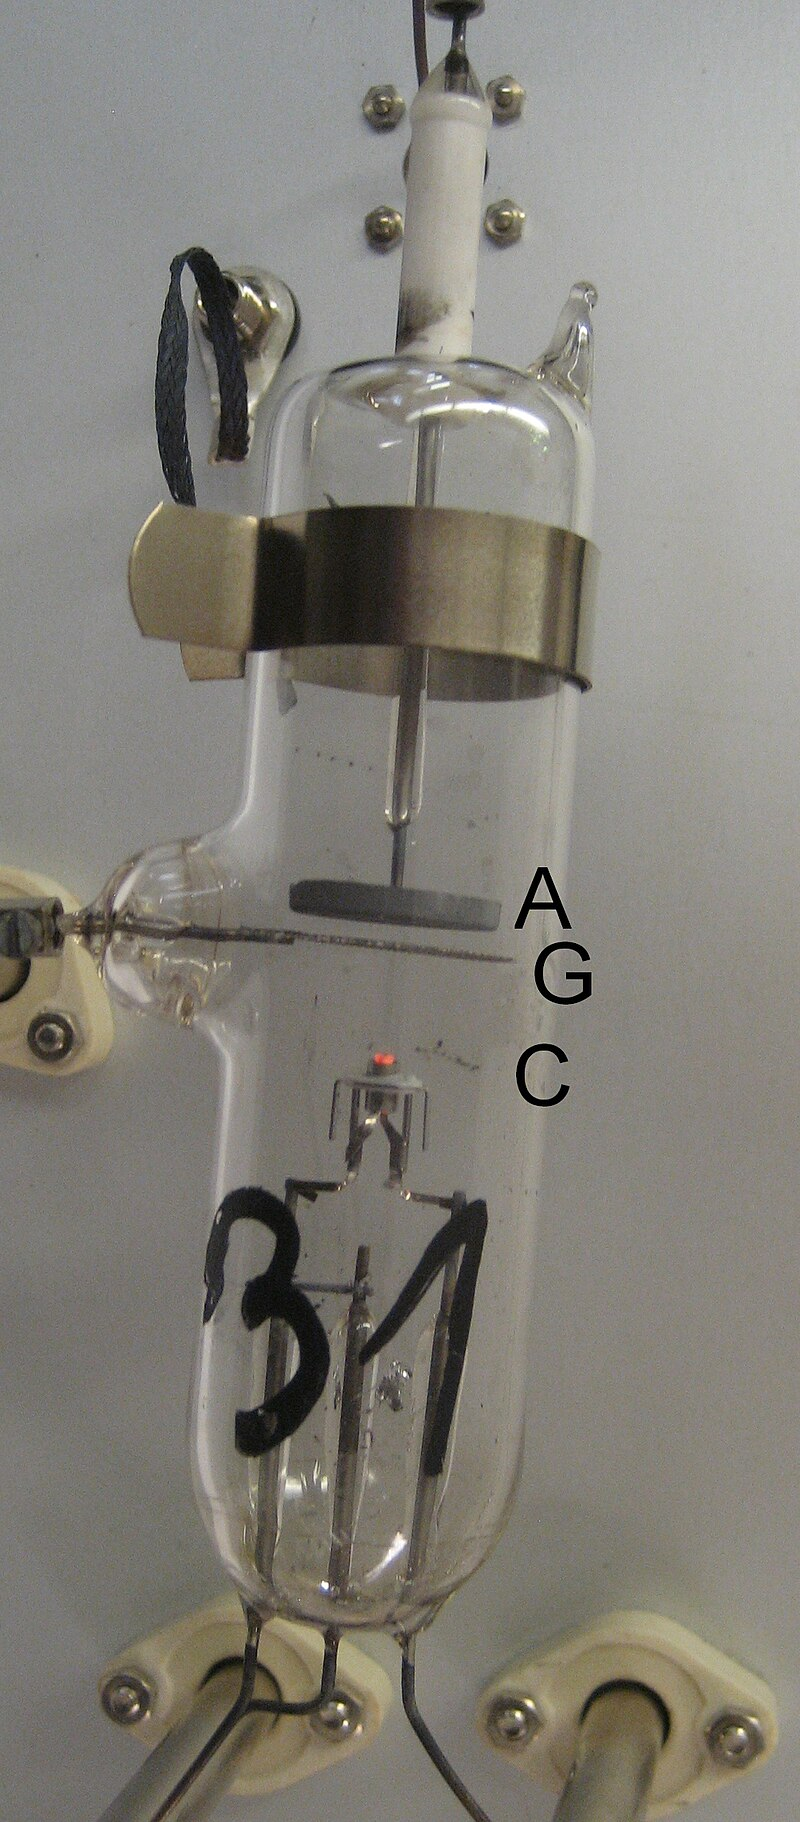
\includegraphics[height=0.5\textwidth]{FranckHertzHgTube}
  \vspace{-10pt}
  \caption{Vakuumska cev koriscena za Frank-Herzov eksperiment}
\end{wrapfigure}
Oko 1900. nekolicina istraživača (Tomson, Tesla, Braun ...) predlagala su promene na Marconijev dizajn. Najverovatnije je Duddelov rad u kojem je koristio rezultate nemačkog naučnika Simona. \newline
Nekoliko godina kasnije, Poulsen je unapredio Duddelov oscilator, i kao takvog ga je prestavio 1906. kao uredjaj za bežični prenos telefonskog govora.\cite{Oscilator}\newline
Prve ideje za nov uredjaj predstavio je Fleming 1904. Za izum ove vakuumske cevi (Flemingov detektor), koristio je rezultate iz oblasti emisije i transporta elektrona u vakuumu, iako detalji fizike nisu bili poznati tada. Modulacija struje u Flemingovoj cevi bila je moguća dodavanjem kontrolne mreže izmedju katode i anode.
Iste godine Lieben je predstavio patent triode sa pojačavačem, koji je i poboljšao 1910 zajedno sa Reiszom i Strausom.
Prvi primer elektronskog oscilatora sa ventilom, nastao je izmedju 1912. i 1913. gde razlika izmedju De Forestovog audiona (prva pojačavačka vakuumska cev) i Lieben-Reiszovog ventila nije razmatrana.\newline
Kako ovi oscilatori nisu funkconisali dobro na frekvencijama iznad 300Mhz, pojavili su se drugi oscilatori, bazirani na vakuumskim cevima u kojima su se vise elektrona slalo u jednom trenutku. 
Prvi slučaj je Barkhausen–Kurz oscilator (1920), koja je funkcionisala u frekvencijama od 300Mhz do 3Ghz. 
Najpopularniji oscilator, bio je klystron (1937) i magnetron (1940). \cite{wikiOsc}
Barkhauzen pokazao je da svi linearni oscilatori moraju da imaju negativnu otpornost.
Balthasar van der Pol je 1927. godine izvršio analizu nelinearnog oscilatora, Van er Pol oscilatora, i time stvorio termin "relaksacioni oscilator" i napravio razliku izmedju linearnih i relaksacionih oscilatora.\newline
Dalje analize oscilatora su bile od strane Hendrik Wade Boda i Harry Nyqista 1930tih. 
Kaneyuki Kurokawa je 1969. godine izveo uslove za oscilaciju u kolima sa negativnim otpornostima, od kojih su nastali moderni mikrotalasni oscilatori\cite{wikiOsc} koji se koriste u komunikacionim sistemima,radarima i veoma brzim digitalnim sistemima.
\newpage
\noindent\makebox[\linewidth]{\rule{0.8\paperwidth}{.4pt}}
\section{Multivibratori i timer555}
\subsection{Multivibratori}
Prvi multivibrator, klasični astabilni multivibrator je prvi put bio opisan od strane Henrija Abrahama i Eugena Bloch-a u dvadesetsedmoj publikaciji "French Ministère de la Guerre" i u "Annales de Physique 12, 252" 1919-te godine. 
Pošto je proizvodilo kvadratni impuls, za razliku od od sinusnih oblika drugih oscilatora, njegov izlaz sadržao je mnogo harmonika iznad osnovne frekvencije,  koji su korišćeni za kalibraciju visokofrekventnih radio kola. Zbog ovog razloga Abraham i Bloch su ga nazvali multivibrator. Preteča je Eccles-Jordan triggera koje je nastalo godinu dana nakon.\cite{multivibrator}
\begin{figure}[ht]
  \centering
  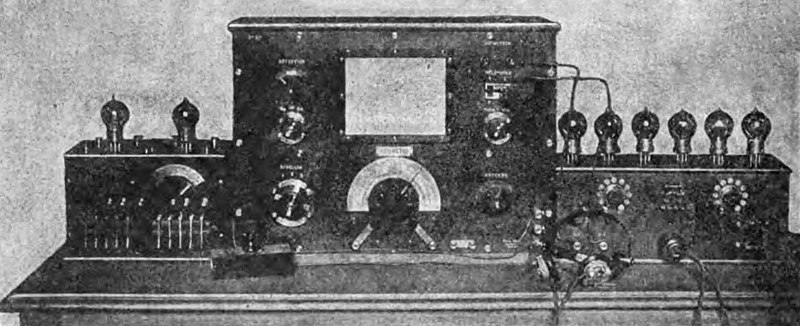
\includegraphics[width=0.7\textwidth]{vakum}
  \caption{Abraham-Bolch multivibrator, Francuska, 1920.}\cite{multivibrator}
\end{figure}

Otprilike u isto vreme, u Velikoj Britaniji, Eccles i Jordan su radili na metroloskom problemu i razvili su kolo koje vibrira zvučnu viljušku. 
Njihovo kolo ima isti "oblik" kao i Abrahamovo i Bolchovo.\newline
\begin{figure}[hb]
  \centering
  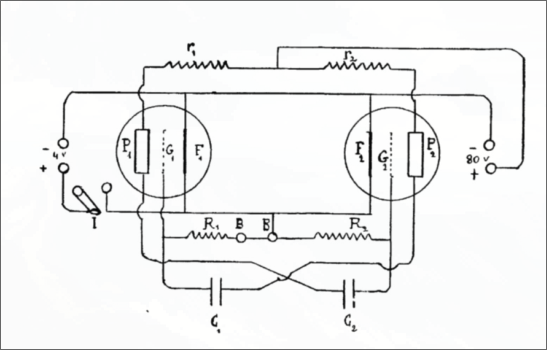
\includegraphics[width=0.5\textwidth]{AB.png}
  \caption{Abrahamovo i Bolchovo kolo}\cite{wVib}
\end{figure}
\begin{figure}[ht]
  \centering
  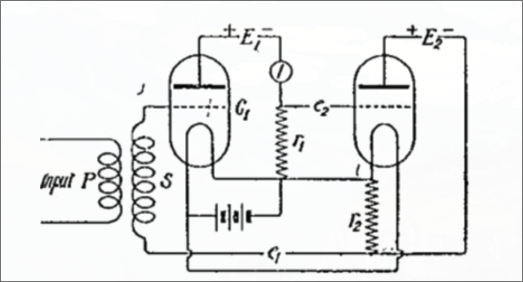
\includegraphics[width=0.5\textwidth]{EJ.png}
  \caption{Ecclesovo i Jordanovo kolo}\cite{wVib}
\end{figure}

Kako su tube vezane optornicima a ne kondenzatorima, kolo nema dinamičo ponašanje. 
Ali ako ne zanemarimo parazitne kapacitivnosti kola, postoje dva dinamička stanja.\cite{wVib}
Samim tim njihovo kolo se zvalo flip-flop. Takodje je 1920. Laurence B. Turner predstavio slično kolo pod nazivom "Kallirotron".
Abrahamovo i Bolchovo kolo je bilo razmatrano sve do kasnih 30-tih, ali je postepeno izgubilo svoju svrhu.\newline
Na žalost, njihov naučni potencijal bio je ugašen 1943. godine, kada su Abraham i Bolch bili pogubljeni gasom, u nemačkom Aushwitz-Birkenau koncentracionom logoru.\newline 





Multivibratori se dele na:
\begin{itemize}
  \item Astabilni Multivibratori
  \item Monostabilni Multivibratori
  \item Bistabilni Multivibratori
\end{itemize}
Astabilni multivibrator je kolo koje nije stabilno u ni jednom stanju. 
Konstantno prelazi iz jednog stanja u drugo. Radi kao relaksacioni oscilator. 
\newline
Monostabilni multivibrator je kolo čije je jedno stanje stabilno a drugo stanje je nestabilno (tranzijentno). Trigger impuls izaziva da kolo predje u tranzijentno stanje, nakon dolaska u to stanje, nakon nekog vremena kolo se vraca u stabilno stanje. 
\newline
Bistabilni multivibratori je kolo koje stabilno u oba stanja. Može da predje iz jednog stanja u drugo pomoću spoljašnjeg trigger impulsa. Ovo kolo je takodje poznato kao flip-flop ili leč kolo. Može da sadrži jedan bit informacije, često se koristi kod računarske memorije. 
Multivibratori se koriste u raznim oblastima i sistemima gde su potrebni pravougaoni impulsi ili tačno odmereni vremenski intervali. Na primer u ranim televizijskim sistemima.
\newpage
\noindent\makebox[\linewidth]{\rule{0.8\paperwidth}{.4pt}}
\subsection{timer555}
Hans R. Camenzind dizajnirao je prvo 555 timer kolo 1971. godine u Američkoj kompaniji Signetics Corporation.
\begin{wrapfigure}{l}{0.25\textwidth}
  \begin{center}
    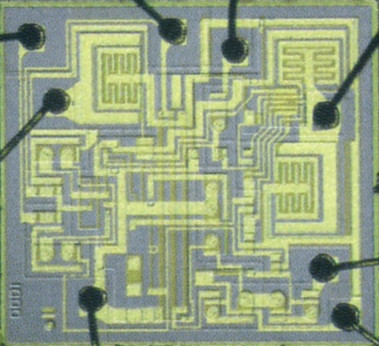
\includegraphics[width=0.2\textwidth]{555si}
  \end{center}
  \caption{prvo 555 IC}\cite{555W}
\end{wrapfigure}
Zapošljen je da dizajnira PLL integrisano kolo, dizajnirao je oscilator za PLL tako da njegova frekvencija nije zavisila od napona napajanja ili temperature. 
Kako je 1970. bila ekonomska recesija, pola radnika Signeticsa dobilo je otkaz i samim tim razvitak PLL kola bio je zaustavljen. 
Camenzid je zatražio da nastavi razvitak svog oscilatora. Samim tim 1971. godine prototip se pojavljuje sa 9 pinova i konstantim izvorom struje. 
Kako je video da je ulazna otpornost sasvim dovoljna za rad kola, smanjio je broj pinova sa 9 na 8, i samim tim smanjio pakovanje sa četrnaestopinskog na osmopinski paket.\cite{555W}
Drugi dizajn imao je 8 pinova, 25 tranzistora, 2 diode i 15 otpornika. Signetics korporacija 1972. je pustila 555 u prodaju u osmo-pinskoj DIP i osmo-pinskoj TO5 metalni paket varijanti. Kako je bilo jedino integrisano kolo u prodaj, takodje jeftino i svestrano, bilo je instantan hit.\cite{555H}
Mnoge knjige pišu da je kolo dobilo ime po tri otpornika od po 5k\ohm, ali kolo je zapravo dobilo ime "555" samo radi marketinga. 
Timer555 integrisano kolo koristi se kao tajmer, oscilator ili pulsni generator.
\begin{figure}[hb]
  \centering
  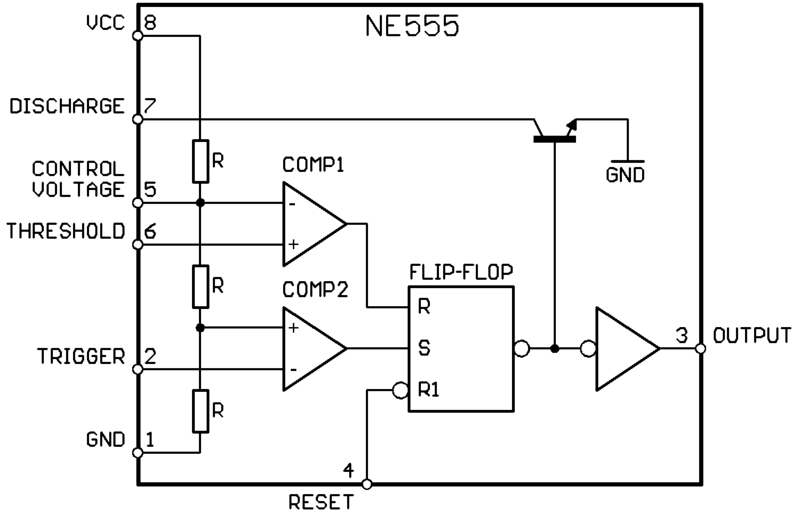
\includegraphics[width=0.65\textwidth]{555}
  \caption{Šema 555 tajmera}\cite{555W}
\end{figure}


\newpage

\noindent\makebox[\linewidth]{\rule{0.8\paperwidth}{.4pt}}
\section{TTL, ECL i CMOS}
Ljudska pohlepa nema kraja, pa nema ni želja da se stane sa razvojem digitalnih kola.\newline
Samim tim je nastao "High-speed" TTL (74H) koji je imao duplo veću brzinu i duplo veću snagu (smanjujući vrednosti otpronika na pola) .\cite{art}
Druga familija, ECL (emitter-coupled logic), dostavila je prave brzine (30MHz), koristeći negativno napajanje i malu razliku medju logičkim nivoima (-0.9V i -1.75V); konzumirala je dosta snage (30mW/kapiji) i dolazile je samo u malim integrancijama.
Za manje snage koristio se TTL 74L serije. 
Nazad u RCA (Radio Corporation of America), prvi od MOSFET logičke familije, bio je razvijen, 4000 serija CMOS.Imao je veoma malu potrošnju u stanju mirovanja i širok opseg napajanja (+3V do +12V). Ulazna struja bila je približna nuli ali je brzina kola bila očajna i kola su bila dosta skupa.
Tokom 1970-tih TTL dobija "Schottky-clamped" familije: prvo 74S seriju koja je načinila 74H bespotrebnim (tri puta veća brzina za dva puta veću snagu), kasnije je 74LS obezvredio standardnu 74-seriju, pružajući malo veće brzine za 1/5 snage svoga prethodnika. 
Fairchild je ubrzo osmislio 74F (F for FAST: "Fairchild Advanced Schottky TTL") koje je i do 50\% brže od 74S a 1/3 manje troši od njega.
\begin{figure}[ht]
  \centering
  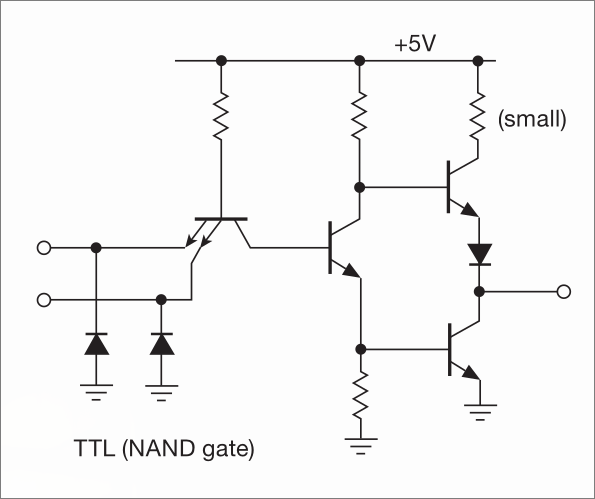
\includegraphics[width=0.5\textwidth]{TTL(NAND).png}
  \caption{TTL(NAND) kolo}\cite{art}
\end{figure}
\newline
Texas instruments izbacio je svoju 74AS ("Advanced Schottky") i 74ALS (low power verziju) čija je namena bila da zameni 74S i 74LS, respektivno. 
Sve ove TTL familije imaju iste logičke nivoe (iste vrednosti napona za '0' i '1') i izlazni napon, pa su mogli da se kombiniju u istom kolu.\cite{art}
U medjuvremenu, 4000 serija CMOS je prešla u 4000B seriju, sa još većim opsegom ulaznih napona (+3V do +18V), boljom ulaznom zaštitom i većom brzinom (3.5MHz na 5V). 
ECL je dobio ECL II, ECL III, ECL 10000 i ECL 100000 serije sa brzinama i do 500MHz.
\begin{figure}[h]
  \centering
  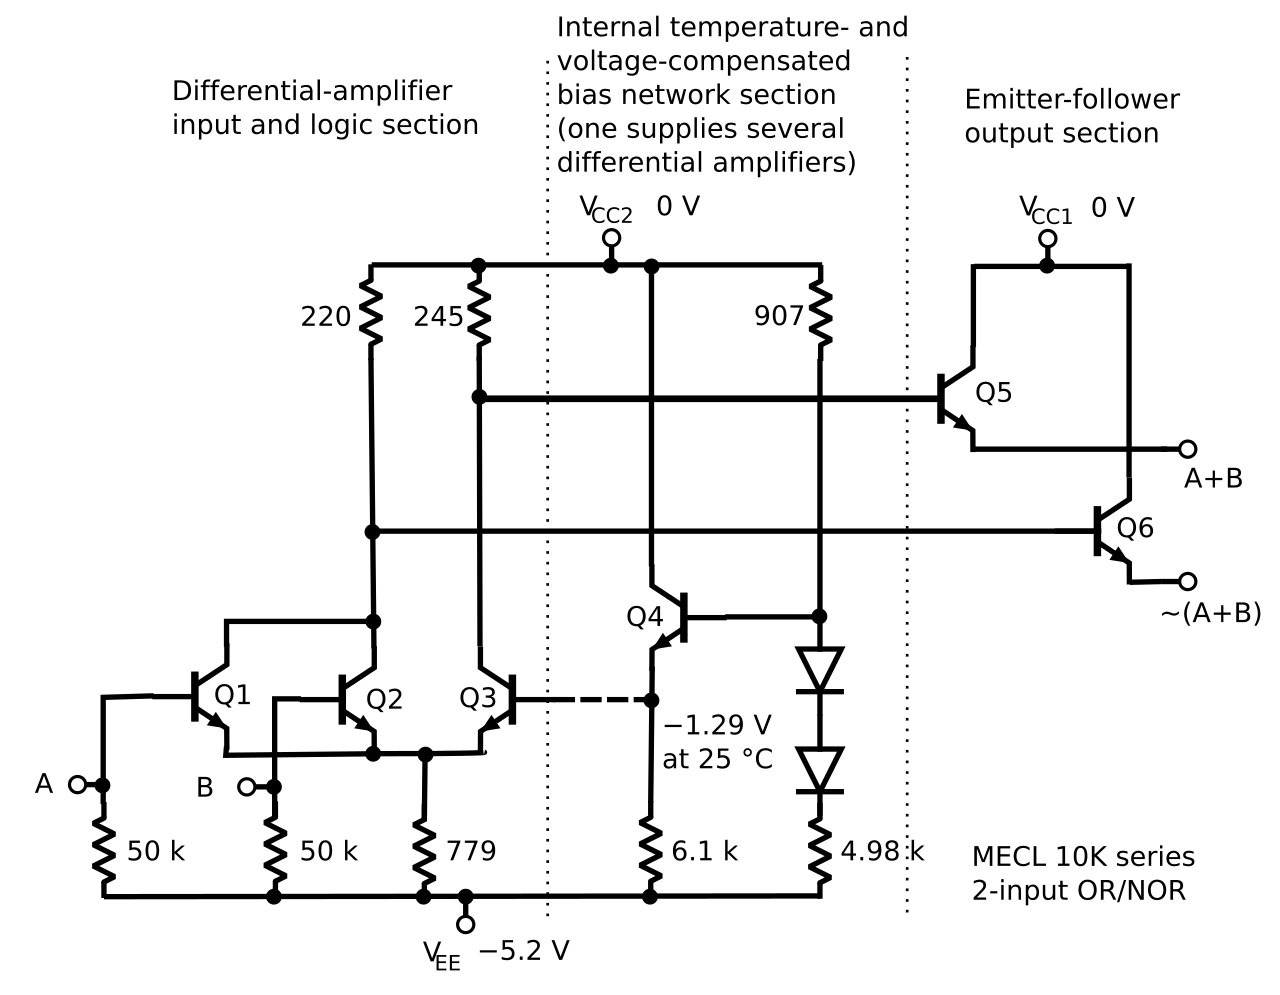
\includegraphics[width=0.75\textwidth]{ECL}
  \caption{Motorola ECL 10000}\cite{ecl}
\end{figure}
Začetkom sledeće decenije većina dizajniranja oko 74LS bila je zasvršena, ubacujući 74F gde god je veća brzina bila potrebna. Ovaj isti TTL bio je korišćen kao "lepak" da poveže nMOS mikroprocesorska kola, čiji su ulazi i izlazi bili TTL kompatibilni. 
Mikroenergetski dizajn je uvek upražnjavao 4000B ili 74C CMOS, ali za veće brzine ECL.

\newpage

Nije bilo dosta mešanja medju familijama, osim ponekih kombinacija CMOS-a i TTL-a, ili TTL-a i ECL kola.

Kako su osamdesete bile u punom jeku, došla je neverovatno razviće CMOS logike, koja se hvalila brzinom i izlaznim naponom TTL kola:
Prvo 74HC ("High-speed CMOS"), sa istom brzinom kao 74LS, i naravno malom potrošnjom, odmah nakon 74AC ("Advanced CMOS") stupa na scenu, sa istom brzinom kao i 74F ili 74AS.
Ova kola sa svojim superiornijim karakteristikama su u suštini zamenila bipolarna TTL kola, medjutim bilo je do problema kompatibilnosti ako su se koristile obe logike u jednom kolu, zbog +2.4V HIGH logike izlaza tradicionalnog TTL kola i ulaza CMOS kola sa minimalnim ulaznim naponom on +3.5V. 
Da bi se ovaj problem razrešio CMOS je pružao varijante sa manjim minimalnim ulaznim naponom: 74HCT i 74ACT. 
Ovu deceniju je takodje označio začetak LSI i VSLI (mikroprocesori, memorije\dots), koji su evoluirali od nMOS do CMOS. Za primene pri velikim brzinama bilo je priče o razvitku GaAs (Galijum-Arsen) logičkih uredjaja koje bi dostigle brzine i do 3GHz.
Bez imalo sumnje tehnologija je dosta napredovala u sledeće dve decenije. 
Najbitniji razvitak bio je u CMOS grani, performanse, koje su se poboljšale smanjivanmjem tehnologije na čipu ("skaliranje"). Smanjivanjem tranzistora je jelte omogućilo povećanje broja istih na čipu, što je dovelo do skoka u razviću raznoraznih tehnologija, poput grafičkih kartica, većih i jačih procesora i memorija\dots 
Rezultat su nove familije CMOS logičkih jedinica (74LVC, 74AUC \dots) koje su dostigle brzine megaherca. 
Većina ovih jedinica funkcioniše na opsegu napona od +1.8V pa do +5V.
Sa porastom VLSI tehnologije, smanjila se potreba za dsikretnom logikom, i ove standardne logičke komponente su se koristle nečesto. Zbog tog razloga dolazile su u malim paketima, sadržujući jednu ili dve kapije, flip-flop sa imenima poput TinyLogic, Little Logic, MiniGate ili PicoGate.
Devedesete su imale problem sa "plutajućim uzemljenjem", koje je TI probao da reši tako što je u sredini kola dodao dodatne pinove za masu i napon (74AC11004); drugi su kreirali "tihe" logičke familije koje su mogle da kontrolišu bzinu promene takta. 
Situacija se veoma popravila prelaskom na manje napona napajanja, SMT i dobra rasporedjivanje elementa po PCB-u.
Korišćenje LVDS (low-voltage differntial signaling) za brze signale je skoro pa eliminisalo problem.



\newpage
\section{Moderni procesor}

\newpage

\printbibliography[title={Reference}]
\end{document}

